\documentclass{article}[10pt]

\usepackage{graphicx}
\usepackage{listings}
\usepackage{xcolor}

\graphicspath{ {img/} }

\definecolor{mygray}{rgb}{0.5,0.5,0.5}

\begin{document}

\title{Logic programming project: square packing}
\author{Lorenzo Corneo, Nikolaos-Ektoras Anestos, Antonios Kouzoupis \\
	\{corneo,anestos,antkou\}@kth.se}
\date{\today}
\maketitle

\section{Introduction}

The purpose of the project is to get a set of solutions for the square packing problem. Its aim is to pack N squares, of increasing dimension (from 1 to N), in the minimum possible surrounding square of size S.

Our implementation does not make use of the constraint functions already existing in Prolog, so the search strategy is driven by the permutations of the all possibles coordinates that can be assigned to every single square. Additionally, we provide some primitive set of constraints, to bind the possible range of coordinates a square can have assigned.

\section{Assumptions}

The program works in two ways. The first way takes as inputs the number of squares and a set of unbound variables that will contain the coordinates of the solution. The size of the optimal surrounding square is not provided as it is automatically found. The used method is naive: we start from S=N and every time the unification fails, S is increased. Eventually, the  optimal S is found and Prolog returns the optimal solution, performing a cut (with an if statement).

The second way takes as input also the size of the surrounding square S. This way, it is possible to verify that for underestimated values of S the program fails. Then, when S is big enough Prolog keeps on listing all the possible solutions to the square packing problem.

We decided to implement also the second way because the first one is very expensive in terms of computation. Actually, with N$>$4 it can take a lot of time to compute the result. The second way it is faster because S is provided and the unification will either fail or return a set of solutions.

In order to improve the first way of functioning, we decided to set $S=2N-1$ which is exactly the size of the minimum surrounding square for N squares. After this improvement, the first way result more efficient because it always comes up with a solution, while the second way might not present a solution when S is underestimated.

\section{Implementation details}

In this Section we will briefly go through our program and provide some insight where necessary. First, the entry point is either \texttt{sqp\_no\_s/2} or \texttt{sqp\_with\_s/3}, providing the functionality described above. Then we have to generate all the possible combinations of coordinates that the squares can be assigned. The function \texttt{gen\_combinations/3} will produce all the possible combinations in the form of [(0,0), (0,1), (1,0), (1,1), $\dots$]. Initially it uses \texttt{gen\_coord/3} to produce a list of  X and Y coordinate numbers upper bounded by the side of the enclosing square, [0, 1, 2, $\dots$, S - 1]. Finally, with \texttt{gen\_comb/4} it produces all combinations.

Then, the function \texttt{n\_from\_m/2} will select and bind possible coordinates to squares. Those coordinates will be mapped to \texttt{sq/2} ADT and will be checked if they meet our requirements. The first check, is whether a pair of X and Y coordinates is valid, formally \texttt{X + L <= MAX\_PERMITTED\_COORD}, where L is the the side of the square in question. The same check is done also for the Y dimension and for all squares. Moving on on our checks, two squares should never overlap. \texttt{sq\_overlap/1} takes the list of squares with the assigned coordinates and checks whether the assigned coordinates for a square, overlap with any of the others. A code snippet for that function is shown below.

\lstset{
  language=Prolog,
  numbers=left,
  basicstyle=\footnotesize,
  frame=single,
  numberstyle=\tiny\color{mygray},
  breaklines=true
}

\lstinputlisting[caption={No overlapping check}]{sq_overlap.pl}

Finally, the squares with the assigned coordinates might not fit in current S, so we evaluate this with \texttt{check\_sq\_fit/2}. In case where any of the above checks fail, \texttt{n\_from\_m/2} will produce another combination of coordinates and follow the procedure briefly explained above.

\section{Conlcusion}

We conclude reporting the output of the computation for \texttt{N=4}. In Fig. \ref{fig:sqp} a 2D representation of the following solution is provided.

\footnotesize
\begin{verbatim}
?- sqp_with_s(4, [(X0, Y0), (X1, Y1), (X2, Y2), (X3, Y3)], 7).

Size: 4, X: 3, Y: 0
Size: 3, X: 4, Y: 4
Size: 2, X: 2, Y: 4
Size: 1, X: 3, Y: 6
Optimal size: 7
Time is seconds: 54.330326
X0 = X3, X3 = 3,
Y0 = 0,
X1 = Y1, Y1 = Y2, Y2 = 4,
X2 = 2,
Y3 = 6 
\end{verbatim}

\normalsize
\begin{figure}[h]
\centering
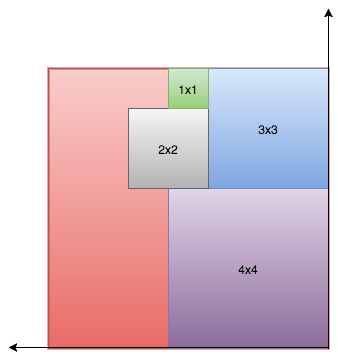
\includegraphics[scale=0.4]{sqpn4}
\caption{2D representation for the solution provided by the program for N=4..}
\label{fig:sqp}
\end{figure}

The elapsed time for getting the result is around 55 sec and it is not really efficient, but the scope of the project is to solve the square packing in a logic programming fashion using Prolog.

\end{document}